\documentclass[11pt,french,french]{article}
\usepackage{lmodern}
\usepackage{amssymb,amsmath}
\usepackage{ifxetex,ifluatex}
\usepackage{fixltx2e} % provides \textsubscript
\ifnum 0\ifxetex 1\fi\ifluatex 1\fi=0 % if pdftex
  \usepackage[T1]{fontenc}
  \usepackage[utf8]{inputenc}
\else % if luatex or xelatex
  \ifxetex
    \usepackage{mathspec}
    \usepackage{xltxtra,xunicode}
  \else
    \usepackage{fontspec}
  \fi
  \defaultfontfeatures{Mapping=tex-text,Scale=MatchLowercase}
  \newcommand{\euro}{€}
\fi
% use upquote if available, for straight quotes in verbatim environments
\IfFileExists{upquote.sty}{\usepackage{upquote}}{}
% use microtype if available
\IfFileExists{microtype.sty}{%
\usepackage{microtype}
\UseMicrotypeSet[protrusion]{basicmath} % disable protrusion for tt fonts
}{}
\usepackage[margin=0.95in]{geometry}
\ifxetex
  \usepackage{polyglossia}
  \setmainlanguage{}
\else
  \usepackage[shorthands=off,french]{babel}
\fi
\ifxetex
  \usepackage[setpagesize=false, % page size defined by xetex
              unicode=false, % unicode breaks when used with xetex
              xetex]{hyperref}
\else
  \usepackage[unicode=true]{hyperref}
\fi
\hypersetup{breaklinks=true,
            bookmarks=true,
            pdfauthor={},
            pdftitle={},
            colorlinks=true,
            citecolor=blue,
            urlcolor=blue,
            linkcolor=magenta,
            pdfborder={0 0 0}}
\urlstyle{same}  % don't use monospace font for urls
\setlength{\parindent}{0pt}
\setlength{\parskip}{6pt plus 2pt minus 1pt}
\setlength{\emergencystretch}{3em}  % prevent overfull lines
\setcounter{secnumdepth}{5}

%%% Use protect on footnotes to avoid problems with footnotes in titles
\let\rmarkdownfootnote\footnote%
\def\footnote{\protect\rmarkdownfootnote}


  \title{Analyse statistique et empirique des modèles\\
de Word Embedding sur Twitter}
    \author{Kim Antunez, Romain Lesauvage, Alain Quartier-la-Tente\\
sous l'encadrement de Benjamin Muller (Inria)}
    \date{}
  
\usepackage{caption}
\usepackage{graphicx}
\usepackage{natbib}
\usepackage[dvipsnames]{xcolor}
\usepackage{fontawesome}
\DeclareMathOperator{\arctanh}{arctanh}
\usepackage{subcaption}

\begin{document}

\maketitle


{
\hypersetup{linkcolor=black}
\setcounter{tocdepth}{3}
\tableofcontents
}
\hypertarget{partie-1}{%
\section{Partie 1}\label{partie-1}}

\label{sec:word2vec}

\hypertarget{uxe9valuation-du-moduxe8le-impluxe9mentuxe9}{%
\section{Évaluation du modèle
implémenté}\label{uxe9valuation-du-moduxe8le-impluxe9mentuxe9}}

\hypertarget{comment-uxe9valuer-le-moduxe8le}{%
\subsection{Comment évaluer le modèle
?}\label{comment-uxe9valuer-le-moduxe8le}}

\label{sec:comment_evaluer}

Malgré l'utilisation généralisée des \emph{word embedding}, très peu de
travaux théoriques expliquent ce qui est réellement capturé par ces
représentations de mots.

C'est pourquoi ce modèle est principalement évalué à l'aide de méthodes
empiriques. Nous allons décrire dans cette partie
\ref{sec:comment_evaluer} quelques méthodes que nous avons retenues pour
évaluer la qualité des vecteurs-mots obtenus.

\hypertarget{distance-entre-deux-mots}{%
\subsubsection{Distance entre deux
mots}\label{distance-entre-deux-mots}}

L'un des enjeux principaux du modèle étant de pouvoir estimer la
proximité entre deux vecteurs-mots, nous pouvons tout d'abord mesurer
cette dernière par des calculs de distance.

Il existe différents types de distances. Chacune d'elles possède des
propriétés intéressantes et s'adaptent plus ou moins bien au problème
traité. Nous avons ici retenu deux distances classiquement utilisées :

\begin{itemize}
\item \textbf{la distance euclidienne} $ d_{e}(\vec{u},\vec{v}) = \left\| \vec{u} - \vec{v}  \right\|_2$

La longueur du vecteur mot, captée dans le cas de la distance euclidienne, est positivement corrélée à la fréquence d'apparition du mot (\cite{Schakel}). Cette information peut s'avérer utile dans l'analyse de la signification des mots, notamment lorsque l'on effectue des opérations sur les vecteurs (comme l'exemple de $\overrightarrow{Paris} - \overrightarrow{France} + \overrightarrow{Italie} = \overrightarrow{Rome}$ dans \cite{Mikolov})

Toutefois, cette dépendance à la fréquence d'apparition peut également fausser l'analyse. C'est pourquoi nous avons choisi, par la suite, de normaliser les vecteurs. 

$ d_{e}(\vec{u},\vec{v}) = \left\| \frac{\vec{u}}{\left\| \vec{u} \right\|_2} - \frac{\vec{v}}{\left\| \vec{v} \right\|_2}  \right\|_2$


\item \textbf{la similarité cosinus} $ d_{c}(\vec{u}, \vec{v}) = \frac{\vec{u}.\vec{v}}{\left\| \vec{u} \right\|_2  \left\| \vec{v} \right\|_2 }$.

La similarité cosinus correspond au produit scalaire entre les deux vecteurs normalisés. Elle mesure ainsi l'angle formé entre deux vecteurs-mots.

C'est la distance que de nombreux papiers fondateurs de la méthode \emph{Word2Vec} (comme \cite{Mikolov} ou \cite{Levy}) utilisent avec l'argument selon lequel les mots apparaissant dans des contextes similaires sont groupés dans la même direction durant l'entraînement. 
Une similarité est proche de +1 si deux mots sont positivement reliés (proches), de -1 s'ils sont négativement reliés (éloignés) et de 0 s'ils ne sont pas \og reliés \fg{}. 

Il est toutefois délicat d'interpréter une similarité proche de -1. On pourrait intuitivement penser à des antonymes, comme \og grand \fg{} et \og petit \fg{}, mais en pratique, les antonymes sont susceptibles d'apparaître dans des contextes semblables et sont donc bien souvent positivement corrélés. 

 
\end{itemize}

\hypertarget{analyse-en-composantes-principales}{%
\subsubsection{Analyse en Composantes
Principales}\label{analyse-en-composantes-principales}}

Une fois le modèle \emph{Word2Vec} entraîné, nous obtenons des
\emph{word-embeddings} pour chacun de nos mots, représentés par des
vecteurs de grandes dimensions (20, 50 ou même supérieures à 100).

Dès lors, il devient complexe de bien observer la proximité entre deux
mots. C'est pourquoi il devient utile de mobiliser des méthodes de
réduction de dimensions comme l'analyse en composantes principales
(ACP). L'objectif premier de cette méthode est en effet de projeter un
nuage de points sur un espace de dimension inférieure afin de rendre
l'information moins redondante et plus visuelle, tout en étant le plus
proche possible de la réalité.

Considérons le cas où nous disposons de \(n\) individus (dans notre cas
les mots) et de \(p\) variables (dans notre cas, leurs composantes ou
dimensions issues du modèle \emph{Word2Vec}). On note \(X = (x_{ij})\)
la matrice de taille \((n,p)\) des données brutes, où \(x_{ij}\)
représente la valeur de la \(j\)-ème variable pour le \(i\)-ème
individu. Afin de donner à chaque individu le même poids, nous centrons
et réduisons les colonnes de notre matrice de données. On notera par la
suite \(Z = (z_{ij})\) la matrice des données centrées et réduites.

La construction des axes de l'ACP est faite par projection orthogonale.
Nous utilisons ici le produit scalaire \(<x,y>_{N} = x\,^t N y\) avec la
métrique \(N = diag(\frac{1}{n},...,\frac{1}{n})\). Ainsi, la projection
orthogonale d'un individu i (vecteur ligne) \(z_i\) sur une droite de
vecteur directeur \(v\) vaut \(^tz_iv\) et les coordonnées de projection
des \(n\) individus valent \(Zv\).

Les vecteurs directeurs des axes sont définis de manière à maximiser la
dispersion du nuage (son inertie) des individus projetés et conserver
ainsi au mieux les distances entre les individus. L'inertie se définit
comme

\[I(Z) = \frac{1}{n} \sum \limits_{i = 1}^n d_{e}^2(z_i,\bar{z}) = \sum \limits_{i = 1}^n var(z^j) = p\]

avec \(d_{e}(z_i,z_{i'})\) la distance euclidienne entre deux individus
\(z_i\) et \(z_{i'}\) :
\(d_{e}(z_i,z_{i'}) = \sum \limits_{j=1}^p (z_{ij} - z_{i'j})^2\)\footnote{Nous
  travaillons ici dans le cadre d'une ACP normée où la matrice \(X\) a
  été centrée puis réduite. La réduction de \(X\) a modifié les
  distances initiales entre individus
  (\(d_{e}(z_i,z_{i'}) \neq d_{e}(x_i,x_{i'})\)). Cela n'aurait pas été
  le cas si la matrice \(Y\) avait été uniquement centrée (ACP non
  normée).}.

On trouve tout d'abord le vecteur directeur \(v_1\) qui orientera le
premier axe de l'ACP grâce au programme suivant :
\[v_1 =\underset{\Vert v \Vert = 1}{\mathrm{argmax~}} Var(Zv) =\underset{\Vert v \Vert = 1}{\mathrm{argmax~}} v\,^t R v \]
où \(R = Var(Z) = \frac{1}{n} Z\,^t Z\) est la matrice des corrélations
entre les p variables. La norme du vecteur \(v\) se calcule dans ce
nouvel espace comme
\(\Vert v \Vert = \sqrt{<v,v>} = v ^tv =\sqrt{ \sum \limits_{i = 1}^p v_i^2}\)

Puis, on choisit \(v_2\) orthogonal à \(v_1\) tel que l'inertie soit
toujours maximisée
\[v_2 =\underset{ \Vert v \Vert = 1,\,v \perp v_1}{\mathrm{argmax}}\;  Var(Zv) \]
En procédant de manière séquentielle, on obtient \(q < r\) axes
orthogonaux avec \(r = rg(Z)\) et \(q\) choisi par le
statisticien\footnote{Différentes méthodes existent afin de déterminer
  le \(q\) optimal, comme la règle de Kaiser ou encore celle du coude.}.

On peut montrer que \(\forall k < q\) :

\begin{itemize}
\item $v_k$ est un vecteur propre associé à la k\ieme{} valeur propre $\lambda_k$ de $R$
\item la composante principale $Zv_k$ est centrée et $V(Zv_k)= \lambda_k$
\item Les $Zv_k$ ne sont pas corrélés entre eux
\end{itemize}

On obtient alors la matrice \(F = ZV\) des nouvelles coordonnées
factorielles des individus, avec \(V = (v_1,\dots,v_q)\) la matrice des
vecteurs propres.

Nous utilisons ici l'ACP en vue d'identifier les individus (ici, nos
mots) qui sont proches. Pour ce faire, il suffit de représenter les
coordonnées factorielles de la matrice \(F\) dans des repères, en
général en 2 dimensions pour une question de lisibilité. Deux mots
apparaissant dans des contextes similaires seront proches sur ce repère
et orientés dans la même direction.

Enfin, pour juger de la qualité de la réduction de dimension, on calcule
souvent la proportion de l'inertie totale expliquée par les \(q\)
premières composantes principales.

\[ \frac{V(F)}{I(Z)} = \frac{\sum \limits_{i = 1}^q \lambda_i}{p}\]

\hypertarget{algorithme-t-distributed-stochastic-neighbor-embedding}{%
\subsubsection{Algorithme t-distributed Stochastic Neighbor
Embedding}\label{algorithme-t-distributed-stochastic-neighbor-embedding}}

Bien que l'ACP soit une première manière de résumer l'information
contenue dans nos vecteurs, elle présente des limites, notamment dans
les vecteurs aux trop grandes dimensions, pour lesquels l'inertie des
premiers axes de l'ACP peut se révéler faible.

Pour combler ces lacunes, un autre algorithme de réduction de dimension
peut être utilisé, celui dit du t-distributed Stochastic Neighbor
Embedding. Contraitement à l'ACP, cet algorithme est stochastique et
non-linéaire et il favorise l'apparition de groupes de mots proches. Sa
philosophie demeure cependant identique : représenter dans un espace à
dimension réduite notre nuage de points de manière à repérer les mots
proches.

La première étape de l'algorithme consiste à calculer les similarités
entre les \(n\) vecteurs-mots \((x_i)_{i=1...n}\). La similarité entre
\(x_i\) et \(x_j\) se mesure comme étant la probabilité conditionnelle
\(p_{j|i}\) de choisir \(x_j\) comme voisin de \(x_i\), si les voisins
étaient tirés au sort selon une loi
\(\mathcal{N}(x_i, \sigma_i)\)\footnote{\(\sigma_i\) doit être calculé
  de manière à adapter la loi conditionnelle aux données. Une faible
  dispersion autour de \(x_i\) entraînera un \(\sigma_i\) faible et
  réciproquement. Il s'agit de trouver le \(\sigma_i\) qui minimise ce
  qui est appelé en théorie de l'information la \og perplexité \fg{},
  c'est-à-dire un indicateur qui décrit à quel point une distribution de
  probabilité réussit à prédire un échantillon.}

\[ p_{j|i} = \frac{\exp({-\frac{(d_e(x_i - x_j))^2}{2\sigma_i^2})}}{\sum_{k \neq i}{\exp({-\frac{(d_e(x_i - x_k))^2}{2\sigma_i^2})}}}\]

La seconde étape de l'algorithme consiste à trouver le nouvel espace de
projection à faible nombre de dimensions. On appellera \(g_i\) les
\(x_i\) projetés dans cet espace que l'on cherche à déterminer. De la
même manière que précédemment, on exprime des probabilité
conditionnelles \(q_{j|i}\) en fonction des \(g_i\) mais qui suivent
cette fois-ci une distribution de \emph{Student} - d'où le nom de
l'algorithme - plutôt qu'une loi gaussienne\footnote{Dans un espace à
  faible dimension, la dispersion des vecteurs est réduite. La
  distribution de Student possède des queues plus épaisses que la loi
  normale, ce qui permet de mieux différencier les vecteurs distants des
  vecteurs similaires.}.

\[ q_{j|i} = \frac{(1+ (d_e(g_i - g_j))^2)^{-1}}{\sum_{k \neq i}{(1+ (d_e(g_i - g_k))^2)^{-1}}}\]

Afin d'obtenir les \(g_i\), on minimise, par descente de gradient, la
divergence de Kullback--Leibler entre les distributions de probabilité P
et Q :

\[KL(P,Q) = \sum_{i \neq j} { p_{ij} \log{\frac{p_{ij}}{q_{ij}}}} \qquad\text{avec}\qquad p_{ij} = \frac{p_{i|j} + p_{j|i}}{2n}\]

Comme dans l'algorithme de l'ACP, l'algorithme de t-SNE nous permet
d'obtenir une nouvelle projection des \(x_i\). Il faut cependant
analyser avec précaution ses résultats. L'algorithme n'étant pas
linéaire, l'interprétation de la taille des \emph{clusters} obtenus ou
de la distance qui les sépare n'est alors pas directe.

\hypertarget{jugement-humain}{%
\subsubsection{Jugement humain}\label{jugement-humain}}

\label{sec:jugement_humain}

Les \emph{word-embedding} obtenus par \emph{Word2Vec} sont censés
regrouper les mots qui apparaissent dans un contexte similaire. Une
dernière façon de vérifier la qualité de nos vecteurs-mots est de les
comparer à un jugement humain. Pour ce faire, nous utilisons la liste de
référence RG-65 pour le français\footnote{Le RG-65 a fait appel à 18
  évaluateurs humains. La base, initialement mobilisée dans un article
  anglophone (\cite{Rubenstein}) a été traduite de l'anglais.}
(\cite{Boumedyen}). Elle contient 65 paires de noms communs (tableau
\ref{table:human_judgement}) évaluées sur une échelle de 0 (non liés) à
4 (très liés).

\begin{table}
\begin{center}
\begin{tabular}{|c|c|c|}
    \hline
    mot 1 & mot 2 & similarité  \tabularnewline
    \hline
    corde & sourire & 0,00   \tabularnewline
    midi & ficelle & 0,00   \tabularnewline
    \dots & \dots & \dots   \tabularnewline
    corde & ficelle & 3,33   \tabularnewline
    \dots & \dots & \dots   \tabularnewline
    automobile & auto & 3,94   \tabularnewline
    coq & coq & 4,00   \tabularnewline
    \hline
 \end{tabular}
\captionsetup{margin=0cm,format=hang,justification=justified}
\caption{Base de données de jugement humain}\label{table:human_judgement}
\end{center}
\end{table}

Nous calculons ensuite la corrélation de Spearman entre les similarités
cosinus de ces différentes paires issues de notre modèle (notées ici
\((X_i)_{i=1..n}\)) et les scores proposés ci-dessus par des êtres
humains (notés ici \((Y_i)_{i=1..n}\)).

La corrélation de Spearman est égale au coefficient de corrélation de
Pearson calculé sur les variables de rang. \[
r_s = \mathrm{corr}(\mathrm{rg}_X, \mathrm{rg}_Y) = 
\frac{\mathrm{cov}(\mathrm{rg}_X, \mathrm{rg}_Y)}{
\sigma_{\mathrm{rg}_X} \sigma_{\mathrm{rg}_Y}
}
\] La variable de rang \(\mathrm{rg}_{X_i}\) est définie telle que
\(\mathrm{rg}_{X_i}=j \iff X_i = X_{(j)}\) (\(X_i\) est la \(j\)ème plus
petite variable).

Pour tester la significativité de ce coefficient, nous utilisons la loi
sous \((H_0)\) de la statistique de test
\(z = \arctanh(r_s) = \frac{1}{2} \ln\frac{1+r}{1-r} \overset{H_0}{\sim}\mathcal{N}(0, \frac{1}{n-3})\)
et obtenons l'intervalle de confiance suivant :

\[
IC_\alpha (r_s) = \left[\tanh\left(z-\frac{q_{1-\frac{\alpha}{2}}}{\sqrt{n-3}}\right),
\tanh\left(z+\frac{q_{1-\frac{\alpha}{2}}}{\sqrt{n-3}}\right)\right]
\] avec \(q_{1-\frac{\alpha}{2}}\) le quantile d'ordre
\(1-\frac{\alpha}{2}\) d'une loi \(\mathcal{N}(0, 1)\).

\hypertarget{evaluation-sur-un-corpus-fictif}{%
\subsection{Evaluation sur un corpus
fictif}\label{evaluation-sur-un-corpus-fictif}}

\label{sec:corpus_fictif}

Avant de nous attaquer au jeu de données complet décrit plus bas, nous
avons évalué un premier corpus fictif afin de nous assurer de la
robustesse du modèle implémenté. Nous avons associé dix couples (du type
{[}voiture, camion{]}), à dix mots contexte différents ({[}véhicule,
moto, \dots{]}). Le corpus fictif est formé de 10 000 phrases composées
chacune d'un mot d'un couple, de cinq mots du contexte et de trois mots
bruits, tous tirés aléatoirement.

Nous avons ensuite mis en œuvre les différentes techniques
d'évaluation\footnote{à l'exception de la méthode par \og jugement
  humain \fg{} puisque le corpus est ici créé fictivement par ordinateur
  sans prêter attention au réel sens des mots.} présentées en partie
\ref{sec:comment_evaluer} sur les \emph{word-embeddings} obtenus grâce à
ce corpus fictif.

\begin{table}
\begin{center}
\begin{tabular}{|c|c|c|}
    \hline
    mot & similarité cosinus \tabularnewline
    \hline
    énorme & 0,991   \tabularnewline
    taille & 0,991   \tabularnewline
    \dots & \dots    \tabularnewline
    vanille & 0,061   \tabularnewline
    salissures & 0,054   \tabularnewline
    \hline
 \end{tabular}
\captionsetup{margin=0cm,format=hang,justification=justified}
\caption{Mots les plus proches de \og grand \fg{} par similarité cosinus}\label{table:tableau_evaluation}
\end{center}
\vspace{-0.3cm}
\footnotesize
\emph{Note : Paramètres utilisés : ep = 50 / lr = 0,01 / w = 5 / dim = 10.}
\end{table}

Les résultats semblent concluants : la similarité cosinus montre bien
une forte corrélation entre les mots focus et contexte du corpus initial
et une faible corrélation avec les mots bruits (tableau
\ref{table:tableau_evaluation}). L'ACP et l'algorithme t-SNE permettent
également de montrer graphiquement cette proximité (figure
~\ref{fig:figure_evaluation}). Les clusters apparaissent de manière plus
évidente avec t-SNE.

\begin{figure}
\begin{center}
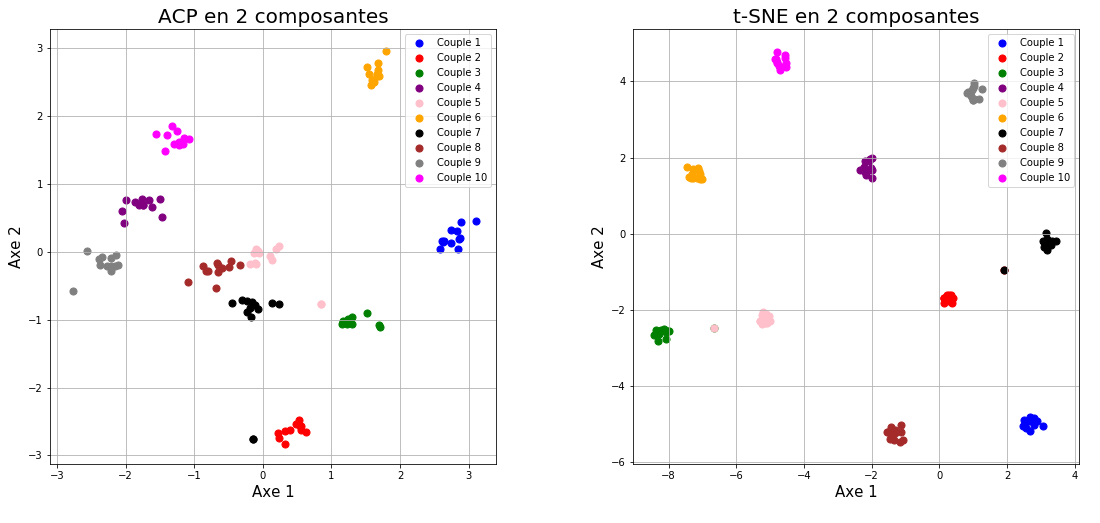
\includegraphics[width=1\textwidth]{img/figures.png}
\captionsetup{margin=0cm,format=hang,justification=justified}
\caption{Évaluation du modèle sur données fictives}\label{fig:figure_evaluation}
\end{center}
\vspace{-0.3cm}
\footnotesize
\emph{Note : Paramètres utilisés : ep = 50 / lr = 0,01 / w = 5 / dim = 10.}
\end{figure}

\hypertarget{choix-des-meilleurs-hyperparamuxe8tres-pour-le-moduxe8le}{%
\subsection{Choix des meilleurs hyperparamètres pour le
modèle}\label{choix-des-meilleurs-hyperparamuxe8tres-pour-le-moduxe8le}}

Une fois nous être assurés de la bonne implémentation du modèle (partie
\ref{sec:corpus_fictif}) grâce au corpus fictif, nous nous sommes
attachés à identifier les hyperparamètres les plus pertinents au regard
des données dont nous disposons.

Ces données correspondent à un ensemble de 1,3 million de
tweets\footnote{Ces tweets, achetés à twitter, sont la propriété de
  l'Inria.} postés en France entre 2014 et 2017, supposés être
représentatifs de l'ensemble de tweets nationaux publiés durant cette
période.

Le modèle \emph{Word2Vec} version CBOW, décrit en partie
\ref{sec:word2vec}, fait en effet intervenir un certain nombre
d'hyperparamètres parmi lesquels :

\begin{itemize}
\item $ep$ : le nombre d'\og \emph{epochs} \fg{}
\item $lr$ ou $\alpha$ : le \og \emph{learning rate} \fg{}, ou taux d'apprentissage
\item $w$ (\emph{window}): la taille de la fenêtre de sélection des mots contextes
\item $dim$ : la dimension des vecteurs-mots (ou \emph{word-embeddings})
\end{itemize}

Or, la performance de nombreuses méthodes de \emph{machine learning},
dont \emph{Word2Vec}, dépend fortement des valeurs choisies pour ces
paramètres, ces valeurs étant elles-mêmes très dépendantes des données
mobilisées.

Même si les méthodes d'optimisation bayésiennes deviennent de plus en
plus performantes pour optimiser la valeur de ces hyperparamètres en
tenant compte de leurs interactions (\cite{Hutter}), ce choix s'effectue
régulièrement de manière empirique, en testant différentes valeurs
d'hyperparamètres sur les données mobilisées. C'est l'approche que nous
retenons ici.

Le package \texttt{Gensim} (\og Generate Similar \fg{}), dans lequel la
méthode \emph{Word2Vec} est implémentée, est un des outils actuels les
plus robustes et performants\footnote{Grâce à sa dépendance à
  \texttt{NumPy}, \texttt{Gensim} puise dans des bibliothèques de bas
  niveau. Ainsi, alors que le code de haut niveau est du Python, c'est
  en fait du Fortran et du C hautement optimisés qui sont utilisés, ce
  qui rend \texttt{Gensim} bien plus performant que \texttt{PyTorch} que
  nous avons utilisé pour implémenter le modèle décrit en partie
  \ref{sec:word2vec}.} pour la modélisation sémantique non supervisée
(\cite{Rehurek}).

Nous avons choisi de mobiliser \texttt{Gensim} dans la suite de ce
rapport, en parallèle du modèle que nous avons implémenté, en raison de
son temps d'exécution bien plus rapide\footnote{A titre d'exemple, alors
  qu'une epoch sur l'ensemble des tweets met une vingtaine d'heures à
  tourner pour \og notre \fg{} modèle, elle met 1 minute via
  \texttt{Gensim}.}. Cette rapidité d'exécution nous a permis de
réaliser des tests d'hyperparamètres plus nombreux.

Pour réaliser ces tests, nous avons fait tourner le modèle
\emph{Word2Vec} plusieurs fois en modifiant un à un les paramètres. Nous
avons ensuite évalué ces différents modèles par la méthode du
\og jugement humain \fg{} (cf.~partie \ref{sec:jugement_humain}) en
comparant la mesure de la similarité cosinus\footnote{Nous avons
  également évalué les modèles en utilisant (l'inverse de) la distance
  euclidienne à la place de la similarité cosinus. L'effet des
  paramètres devient alors bien moins clair et la performance du modèle
  est inférieure, ce va dans le sens de l'utilisation plus fréquente de
  la méthode de la similarité cosinus dans la littérature.} entre deux
mots obtenue à partir de notre modèle à l'évaluation subjective de cette
proximité par des individus. En outre, un même modèle est lancé six fois
(six \og seeds \fg{} différentes) afin de construire des intervalles de
confiance de la matière décrite précédemment, en empilant les six
échantillons de mesure de proximités correspondant aux six
implémentations d'un même modèle\footnote{Pour chaque modèle, nous
  calculons les statistiques de rang des 65 paires de mots de la base de
  jugement humain ainsi que le rang des similarités cosinus des mots
  obtenus en sortie du modèle. Nous réalisons ces actions pour les six
  implémentations du même modèle et empilons les résultats obtenus.
  C'est à partir de cette base empilée de 6x65 lignes moins les données
  manquantes que nous calculons chaque intervalle de confiance selon la
  formule décrite en partie \ref{sec:jugement_humain}.}.

\hypertarget{nombre-depochs-taille-de-fenuxeatre-et-taux-dapprentissage}{%
\subsubsection{Nombre d'epochs, taille de fenêtre et taux
d'apprentissage}\label{nombre-depochs-taille-de-fenuxeatre-et-taux-dapprentissage}}

Pour cette première série de tests d'hyperparamètres, nous avons fixé la
dimension des word-embedding à 50\footnote{En réalisant les mêmes tests
  sur uniquement 100 000 tweets, puis en testant une dimension de
  word-embedding de 20, les effets observés et commentés ici se
  confirment.} et évalué l'impact du nombre d'épochs, de la taille de la
fenêtre et du taux d'apprentissage (figure \ref{fig:evaluation_1}) .

\begin{figure}
\begin{center}
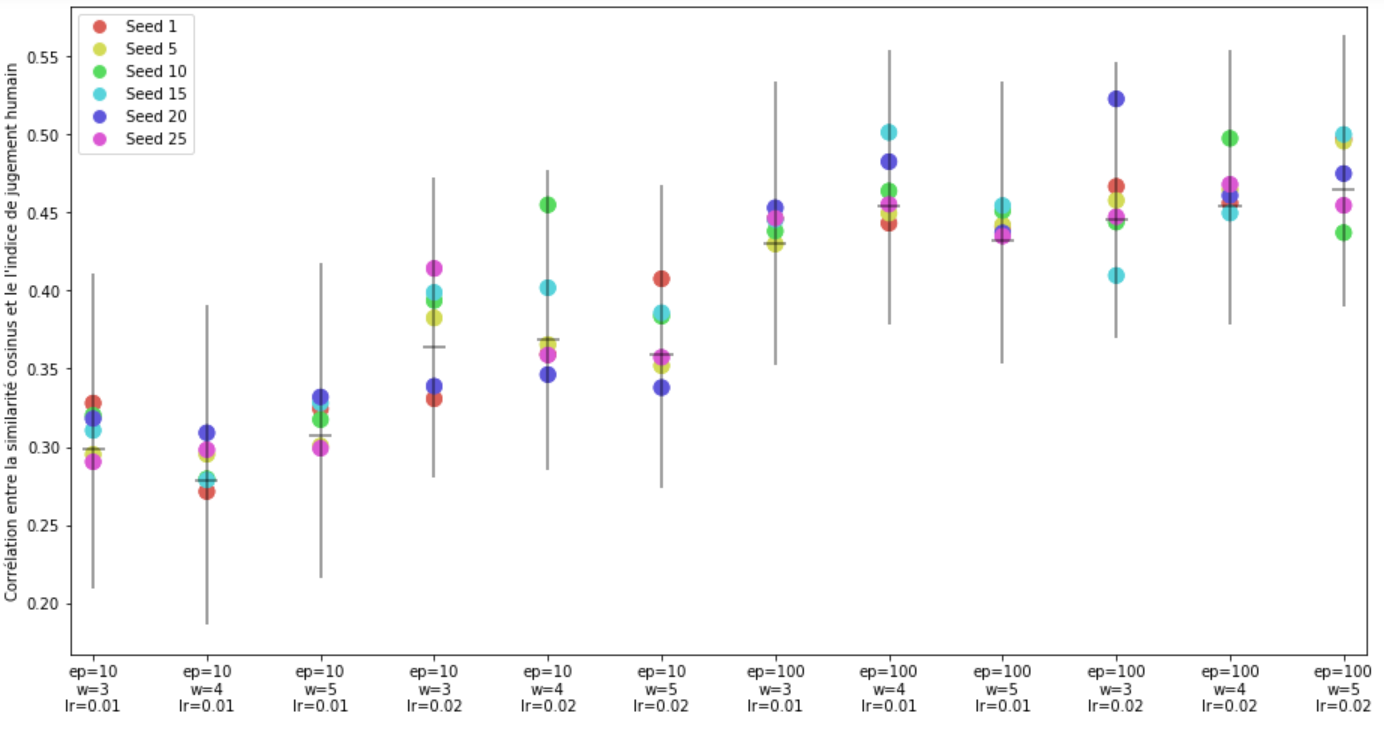
\includegraphics[width=1\textwidth]{img/test_parametres.png}
\captionsetup{margin=0cm,format=hang,justification=justified}
\caption{Tests d'hyperparamètres : epochs, fenêtre et taux d'apprentissage}\label{fig:evaluation_1}
\end{center}
\vspace{-0.3cm}
\footnotesize
\emph{Note : Paramètres utilisés : dim = 50\newline
Le trait horizontal correspond au coefficient de Spearman calculé sur les échantillons empilés des six modèles et la barre verticale à l'intervalle de confiance associé.}
\end{figure}

\hypertarget{le-nombre-depochs}{%
\paragraph{Le nombre d'epochs}\label{le-nombre-depochs}}

~

Le nombre d'epochs à un effet net. Passer de 10 à 100 epochs fait
nettement augmenter le score de corrélation de Spearman entre données
subjectives et données en sortie du modèle.

\faArrowCircleRight{} Nous retenons alors le paramètre \textbf{ep =
100}.

\hypertarget{le-taux-dapprentissage}{%
\paragraph{Le taux d'apprentissage}\label{le-taux-dapprentissage}}

~

La valeur 0,02 semble donner systématiquement de meilleurs résultats que
0,01. En réalisant davantage de tests de taux d'apprentissage en fixant
les autres hyperparamètres, les différents taux d'apprentissage
présentent des performances similaires\footnote{En fixant les paramètres
  dim = 50, ep = 100 et w = 4 (celles du modèle retenu \emph{in fine}),
  et en testant les taux d'apprentissage 0,005, 0,01, 0,02, 0,03 et
  0,04, les valeurs moyennes des corrélations s'échelonnent entre 0,41
  et 0,48, soit des valeurs proches.}.

\faArrowCircleRight{} Nous retenons alors le paramètre \textbf{lr =
0,2}.

\hypertarget{la-taille-de-la-fenuxeatre}{%
\paragraph{La taille de la fenêtre}\label{la-taille-de-la-fenuxeatre}}

~

La taille de la fenêtre ne semble pas jouer un rôle majeur, et dépend
beaucoup des autres paramètres choisis.

Certains travaux (\cite{Levy2}) indiquent que, suivant la taille de
fenêtre choisie, les informations capturées sont différentes. Cela
pourrait expliquer la complexité de choisir la \og meilleure \fg{}
taille de fenêtre. Alors que les \og grandes \fg{} fenêtres capturent
des informations sur le domaine du mot (autres mots de tout type étant
utilisés dans des discussions connexes), les \og petites \fg{} fenêtres
saisissent davantage le mot en lui-même (ses extensions, synonyme, lui
sont alors proches). La valeur de 4 représente une taille de fenêtre
\og ni trop grande ni trop petite\fg{} et qui présente de bons résultats
dans la plupart des tests effectués.

\faArrowCircleRight{} Nous retenons alors le paramètre \textbf{w = 4}.

\hypertarget{dimension-des-vecteurs-mots}{%
\subsubsection{Dimension des
vecteurs-mots}\label{dimension-des-vecteurs-mots}}

On cherche cette fois-ci à évaluer l'effet de la dimension des
\emph{word-embedding}. Selon certains papiers (comme \cite{Pennington}),
la qualité des représentations vectorielles s'améliore à mesure que l'on
augmente la taille du vecteur, mais seulement jusqu'à atteindre 300
dimensions\footnote{La dimension des vecteurs doit également être
  adaptée à la taille du vocabulaire. Un des articles fondateurs de
  word2vec (\cite{Mikolov}) recommande donc d'augmenter à la fois la
  dimension des vecteurs et la quantité de données d'apprentissage. Par
  exemple, avec un vocabulaire d'une centaine de mots, il serait
  inefficace d'utiliser des projections en grande dimension (risque de
  surapprentissage).}. Après 300 dimensions, la qualité des vecteurs
commence à diminuer et le temps de calcul augmente considérablement.

\begin{figure}
\begin{center}
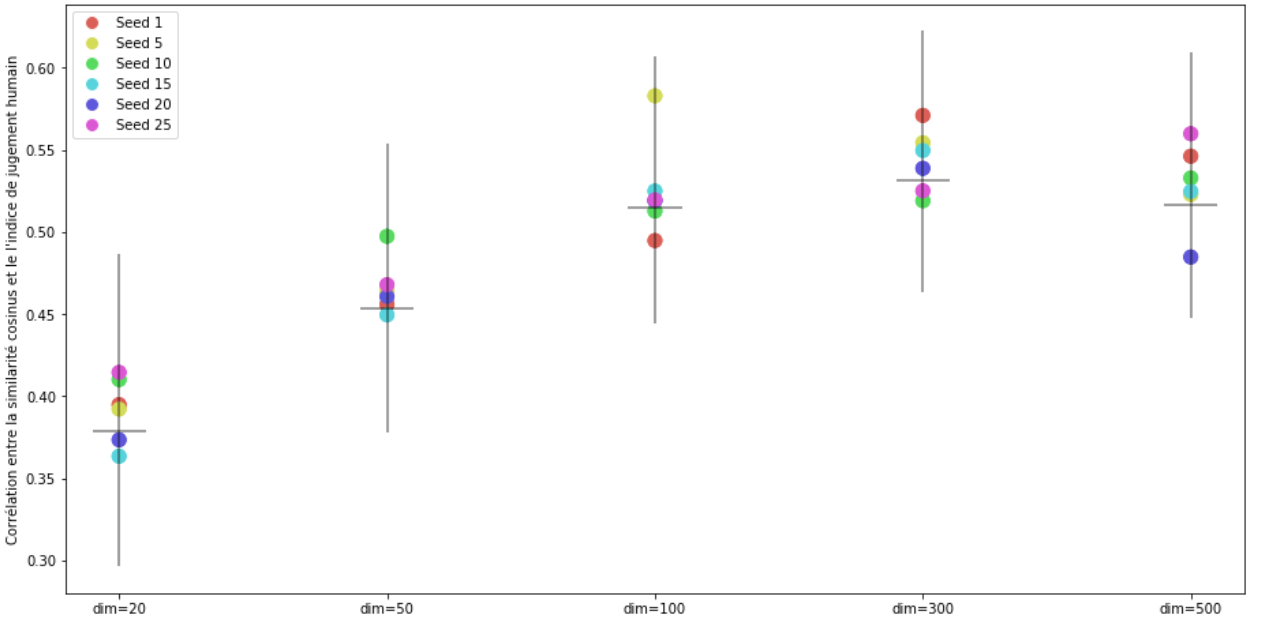
\includegraphics[width=1\textwidth]{img/test_parametres2.png}
\captionsetup{margin=0cm,format=hang,justification=justified}
\caption{Tests d'hyperparamètres : dimension des word-embedding}\label{fig:figure_dim}
\end{center}
\vspace{-0.3cm}
\footnotesize
\emph{Note : Paramètres utilisés : ep = 100 / w = 4 / lr = 0,02.\newline
Le trait horizontal correspond au coefficient de Spearman calculé sur les échantillons empilés des six modèles et la barre verticale à l'intervalle de confiance associé.}
\end{figure}

En pratique, en comparant l'effet de la dimension des vecteurs (modèle
fixé à ep~=~100, w~=~4 et lr~=~0,02), on observe bien une augmentation
de l'efficacité du modèle jusqu'en dimension 300 et une efficacité
moindre en dimension 500 (figure~\ref{fig:figure_dim}). Bien que
l'efficacité du modèle semble meilleure en dimension 300, la dimension
100 améliore la rapidité de l'algorithme, pour des résultats d'une
qualité similaire.

\faArrowCircleRight{} Nous retenons alors le paramètre \textbf{dim =
100}.

\hypertarget{evaluation-sur-le-corpus-final}{%
\subsection{Evaluation sur le corpus
final}\label{evaluation-sur-le-corpus-final}}

\hypertarget{avec-notre-moduxe8le}{%
\subsubsection{\texorpdfstring{Avec \og notre \fg{}
modèle}{Avec notre  modèle}}\label{avec-notre-moduxe8le}}

Nous avons ensuite fait tourner le modèle que nous avons implémenté en
utilisant les paramètres retenus précédemment\footnote{w~=~4, lr~=~0,02
  et dim~=~100} mais uniquement sur 100~000 tweets et 80 epochs pour des
questions de temps de calcul\footnote{près de 18h.}.

Les résultats obtenus semblent relativement satisfaisants. La recherche
des plus proches voisins par similarité cosinus (dont quelques exemples
sont illustrés en tableau \ref{table:knn_ark}) donne des résultats
proches de l'intuition.

\begin{table}
\begin{center}
\begin{tabular}{|c|c|c|c|}
    \hline
\textbf{bonjour} & \textbf{femme} & \textbf{1} & \textbf{samedi} \tabularnewline
\emph{(669 apparitions)} & \emph{(264 apparitions)} & \emph{(765 apparitions)} & \emph{(203 apparitions)} \tabularnewline
       \hline

\includegraphics[height=4mm]{img/emojis/1.png} (0,59) & quelle (0,49) & 5 (0,55) & soir (0,57) \tabularnewline

\includegraphics[height=4mm]{img/emojis/2.png} (0,59) & cette (0,46) & mois (0,51) & vivement (0,51) \tabularnewline
merci (0,54) & une (0,44) & 10 (0,49) & demain (0,50) \tabularnewline
nuit (0,48) & vie (0,44) & 2 (0,48) & end (0,48) \tabularnewline
bisous (0,47) & grippe (0,44) & top (0,48) & weekend (0,47) \tabularnewline
bonne (0,47) & belle (0,43) & depuis (0,47) & matin (0,45) \tabularnewline

\includegraphics[height=4mm]{img/emojis/3.png} (0,46) & ma (0,43) & saison (0,46) & jeudi (0,45) \tabularnewline
vous (0,46) & magnifique (0,43) & ans (0,44) & prochain (0,43) \tabularnewline
plaisir (0,44) & nouvelle (0,43) & jours (0,43) & week (0,43) \tabularnewline
allez (0,43) & vidéo (0,39) & 3 (0,43) & 
\includegraphics[height=4mm]{img/emojis/4.png} (0,42) \tabularnewline
    \hline
 \end{tabular}
\captionsetup{margin=0cm,format=hang,justification=justified}
\caption{10 plus proches voisins par similarité cosinus avec \og notre \fg{} modèle}\label{table:knn_ark}
\end{center}
\vspace{-0.3cm}
\footnotesize
\emph{Note : Paramètres utilisés : ep = 80 / w = 4 / lr = 0,02 / dim = 100 / base : 100 000 tweets\newline
La similarité cosinus de chaque paire de mots est renseignée entre les parenthèses.}

\end{table}

Par ailleurs, le coefficient de Spearman entre la similarité cosinus des
mots obtenus et le jugement humain est de 0,571 (p-valeur : 4,1 \%).
Toutefois, ce bon résultat est à considérer avec précaution puisque
seuls 13 des couples de mots de la base RG-65 ont été reconnus dans le
corpus de 100~000 tweets que nous utilisons ici.

Enfin, les représentations graphiques des positions des mots via des ACP
et les sommes vectorielles sur les mots\footnote{comme l'exemple de
  \(\overrightarrow{Paris} - \overrightarrow{France} + \overrightarrow{Italie} = \overrightarrow{Rome}\)
  dans \cite{Mikolov}} donnent des résultats bien moins concluants que
le modèle \texttt{Gensim} entraîné sur l'ensemble des tweets (cf.~partie
\ref{sec:gensim_resultats})

\hypertarget{avec-le-moduxe8le-gensim}{%
\subsubsection{\texorpdfstring{Avec le modèle
\texttt{Gensim}}{Avec le modèle Gensim}}\label{avec-le-moduxe8le-gensim}}

\label{sec:gensim_resultats}

Le modèle \texttt{Gensim}\footnote{w~=~4, lr~=~0,02, dim~=~100 et
  ep~=~100.} donne des résultats encore plus convaincants que
précédemment, ayant été davantage entraîné, et sur un corpus plus fourni
(ensemble des tweets). En effet, les vecteurs-mots en sortie du modèle
\texttt{Gensim} sur l'ensemble des tweets (figure
\ref{fig:acp_freq_gensim}) sont davantage répartis dans l'ensemble du
plan, alors que les mots en sortie du modèle que nous avons implémenté
sur 100 000 tweets sont répartis en fonction de leur nombre
d'occurrences, les mots les moins fréquents n'ayant probablement pas (ou
peu) été entraînés (figure \ref{fig:acp_freq_ark}).

\begin{figure}
\begin{minipage}{.5\textwidth}
  \centering
  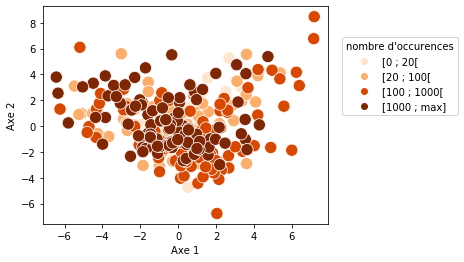
\includegraphics[width=1\linewidth]{img/acp_freq_gensim.png}
  \captionof{figure}{Position des mots en fonction de\newline leur nombre d'occurrences (Modèle \texttt{Gensim})}
  \label{fig:acp_freq_gensim}
\end{minipage}%
\begin{minipage}{.5\textwidth}
  \centering
  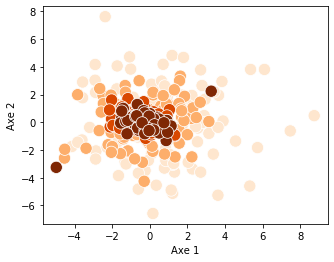
\includegraphics[width=0.72\linewidth]{img/acp_freq_ark.png}
  \captionof{figure}{Position des mots en fonction de\newline leur nombre d'occurrences (\og notre \fg{} modèle)}
  \label{fig:acp_freq_ark}
\end{minipage}
\footnotesize
\emph{Note : Paramètres utilisés : ep = 100 (gauche) ou 80 (droite) / w = 4 / lr = 0,02 / dim = 100.\newline
Méthode utilisée : ACP, deux premiers axes.}
\end{figure}

Le coefficient de Spearman a une valeur semblable à précédemment : 0,495
mais sa p-valeur est proche de 0 \% et, cette fois-ci, 52 des couples de
mots de la base RG-65 ont été reconnus dans le corpus de tweets.

Les 10 plus proches voisins calculés par similarité cosinus (tableau
\ref{table:knn_gensim}) semblent encore davantage pertinents. Les plus
proches voisins de \og \(1\) \fg{} contiennent davantage de chiffres, de
\og samedi \fg{} davantage de jours de la semaine et le tableau contient
désormais des synonymes de \og femme \fg{} et de \og bonjour \fg{}.
Certains mots surprenants subsistent toutefois, comme par exemple
\og transmets \fg{}, \og désagrément \fg{} et \og betembourg \fg{},
voisins de \og bonjour \fg{}. Toutefois, la fréquence d'apparition de
ces mots dans le corpus est faible (moins d'une centaine d'occurrences).
La projection de certains vecteurs-mots sur les deux premiers axes d'une
ACP (figure \ref{fig:acp_gensim}) nous confirme la qualité de
l'entraînement du corpus sur l'ensemble de tweets.

\begin{table}
\begin{center}
\begin{tabular}{|c|c|c|c|}
    \hline
\textbf{bonjour} & \textbf{femme} & \textbf{1} & \textbf{samedi} \tabularnewline
\emph{(17 043 apparitions)} & \emph{(6 177 apparitions)} & \emph{(21 055 apparitions)} & \emph{(4 917 apparitions)} \tabularnewline
       \hline
bonsoir (0,85) & fille (0,86) & 2 (0,65) & vendredi (0,88) \tabularnewline
bjr (0,75) & copine (0,74) & 3 (0,64) & jeudi (0,86) \tabularnewline
hello (0,71) & meuf (0,71) & 6 (0,63) & lundi (0,83) \tabularnewline
salut (0,66) & demoiselle (0,66) & 4 (0,62) & mercredi (0,83) \tabularnewline
coucou (0,55) & nana (0,66) & 7 (0,60) & dimanche (0,83) \tabularnewline
transmets (0,49) & nièce (0,66) & 5 (0,58) & mardi (0,76) \tabularnewline
désagrément (0,48) & sœur (0,65) & 9 (0,58) & demain (0,72) \tabularnewline
avezvous (0,48) & barbe (0,65) & 8 (0,56) & barathon (0,56) \tabularnewline
bettembourg (0,48) & maman (0,64) & 1e (0,55) & 22h45 (0,55) \tabularnewline
hey (0,47) & princesse (0,64) & 34 (0,53) & 20h (0,54) \tabularnewline
    \hline
 \end{tabular}
\captionsetup{margin=0cm,format=hang,justification=justified}
\caption{10 plus proches voisins par similarité cosinus avec le modèle \texttt{Gensim}}\label{table:knn_gensim}
\end{center}
\vspace{-0.3cm}
\footnotesize
\emph{Note : Paramètres utilisés : ep = 100 / w = 4 / lr = 0,02 / dim = 100 / base : ensemble des tweets\newline
La similarité cosinus de chaque paire de mots est renseignée entre les parenthèses.}
\end{table}

\begin{figure}
\begin{center}
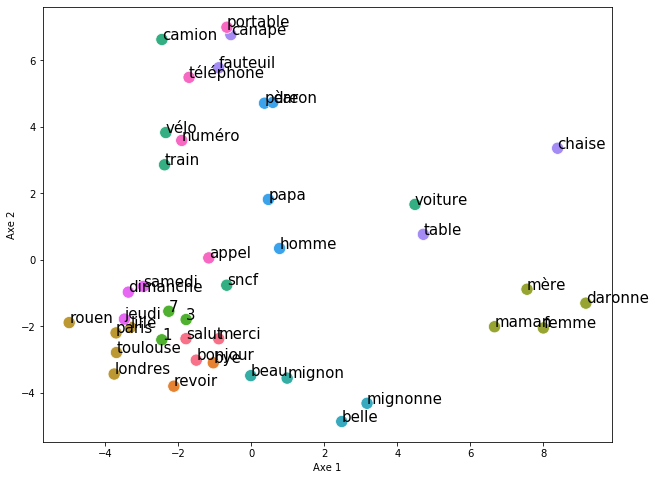
\includegraphics[width=0.5\textwidth]{img/acp_gensim.png}
\captionsetup{margin=0cm,format=hang,justification=justified}
\caption{ACP sur un corpus réduit de mots}\label{fig:acp_gensim}
\end{center}
\vspace{-0.3cm}
\footnotesize
\emph{Note : Paramètres utilisés : ep = 100 / w = 4 / lr = 0,02 / dim = 100 / base : ensemble des tweets }
\end{figure}

Enfin, nous avons réalisé des opérations sur les mots-vecteurs. Si
l'opération
\(\overrightarrow{Roi} - \overrightarrow{Homme} + \overrightarrow{Femme} = \overrightarrow{Reine}\)
(figure \ref{fig:acp_reine}) semble fonctionner\footnote{Les similarités
  cosinus obtenues sont les suivantes :
  \(corr(\overrightarrow{Roi}, \overrightarrow{Homme}) = 0,34\),
  \(corr(\overrightarrow{Homme}, \overrightarrow{Femme}) = 0,35\) et
  \(corr(\overrightarrow{Roi} - \overrightarrow{Homme} + \overrightarrow{Femme} , \overrightarrow{Reine}) = 0,67\).
  \(\overrightarrow{Reine}\) est bien le mot le plus proche de la somme
  vectorielle calculée.}, l'opération
\(\overrightarrow{Paris} - \overrightarrow{France} + \overrightarrow{Italie}\)
(cf. \cite{Mikolov}, figure \ref{fig:acp_rome}) d'identifie pas \og Rome
\fg{} dans les mots les plus proches mais d'autres villes comme \og Lyon
\fg{} (similarité cosinus de 0,62). \og Rome \fg{} semble effectivement
située \og trop en haut\fg{} dans le plan de l'ACP par rapport aux
autres villes. Peut-être ce mot n'a-t-il pas suffisamment été entraîné
(246 apparitions dans les tweets contre 46433 pour Lyon par exemple)
pour que le vecteur-mot obtenu soit pertinent, ou peut-être que, dans
les tweets mobilisés, le mot \og Rome \fg{} s'utilise dans un contexte
différent de l'article de Mikolov.

\begin{figure}
\begin{minipage}{.5\textwidth}
  \centering
  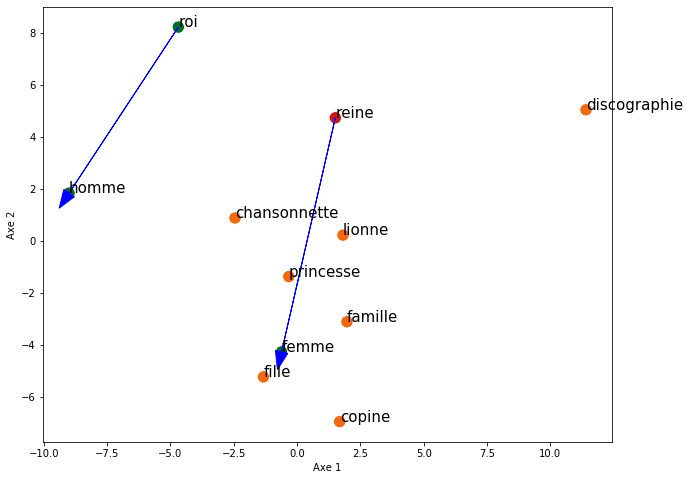
\includegraphics[width=0.92\linewidth]{img/acp_reine.png}
  \captionof{figure}{\ $\protect\overrightarrow{Roi} - \protect\overrightarrow{Homme} + \protect\overrightarrow{Femme} = $ ?}
  \label{fig:acp_reine}
\end{minipage}%
\begin{minipage}{.5\textwidth}
  \centering
  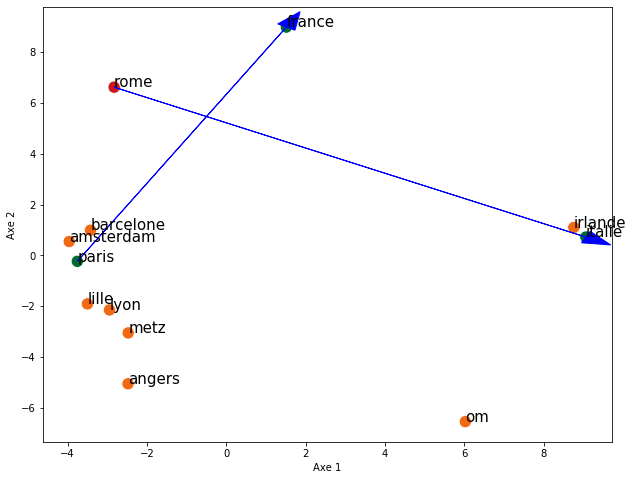
\includegraphics[width=0.85\linewidth]{img/acp_rome.png}
  \captionof{figure}{\ $\protect\overrightarrow{Paris} - \protect\overrightarrow{France} + \protect\overrightarrow{Italie} = $ ?}
  \label{fig:acp_rome}
\end{minipage}
\footnotesize
\emph{Note : Paramètres utilisés : ep = 100 / w = 4 / lr = 0,02 / dim = 100.\newline
Les mots en vert correspondent à ceux présents dans l'opération, le mot en rouge le mot que l'on serait supposé trouver et les mots en orange les 10 mots les plus proches du résultat de l'opération vectorielle.}
\end{figure}

\newpage

\nocite{*}

\begin{thebibliography}{999}
\bibitem[Boumedyen Billami \& Gala (2017)]{Boumedyen} Boumedyen Billami, M.,  Gala, N (2017). Création et validation de signatures sémantiques : application à la mesure de similarité sémantique et à la substitution lexicale. TALN 2017. \url{https://hal.archives-ouvertes.fr/hal-01528117/document}.
\bibitem[Hutter, Hoos \& Leyton-Brown (2014)]{Hutter} Hutter, F., Hoos, H., Leyton-Brown, K., (2014). An Efficient Approach for Assessing Hyperparameter Importance. PMLR 32(1):754-762. \url{http://proceedings.mlr.press/v32/hutter14.pdf}.
\bibitem[Levy \& Golberg (2015)]{Levy} Levy, O., Golberg, Y. (2015). Neural Word Embedding as Implicit Matrix Factorization.
\url{https://papers.nips.cc/paper/5477-neural-word-embedding-as-implicit-matrix-factorization.pdf}.
\bibitem[Levy \& Golberg (2014)]{Levy2} Levy, O., Golberg, Y. (2014). Dependency-based word embeddings. ACL. \url{http://papers.nips.cc/paper/5477-neural-word-embedding-as-implicit-matrix-factorization.pdf}.
\bibitem[Mikolov, Chen, Corrado \emph{et al} (2013)]{Mikolov} Mikolov, T.,  Chen, K., Corrado, G., Dean, J. (2013). Efficient Estimation of Word Representations in Vector Space. arXiv:1301.3781. \url{https://arxiv.org/pdf/1301.3781.pdf}.
\bibitem[Pennington, Socher \& Manning (2014)]{Pennington} Pennington, J., Socher, R., Manning, C. D., (2014).  Glove: global vectors for word representation. Proc. of EMNLP,1532 – 1543. \url{https://www.aclweb.org/anthology/D14-1162.pdf}.
\bibitem[{\v R}eh{\r u}{\v r}ek \& Sojka (2010)]{Rehurek} {\v R}eh{\r u}{\v r}ek, R.,  Sojka, P. (2010). Software Framework for Topic Modelling with Large Corpora. Proceedings of LREC 2010 workshop New Challenges for NLP Frameworks. p. 46--50, 5 pp. ISBN 2-9517408-6-7. \url{https://is.muni.cz/publication/884893/en}.
\bibitem[Rubenstein \& Goodenough (1965)]{Rubenstein} Rubenstein, H.,  Goodenough, J. B. (1965). Contextual Correlates of Synonymy. Commun. ACM, 8 (10), 627–633. \url{https://dl.acm.org/doi/10.1145/365628.365657}.
\bibitem[Schakel \& Wilson (2015)]{Schakel} Schakel, A. M., Wilson, B. J. (2015). Measuring Word Significance using Distributed Representations of Words. arXiv:1508.02297. \url{https://arxiv.org/pdf/1508.02297v1.pdf}.
\end{thebibliography}

\end{document}